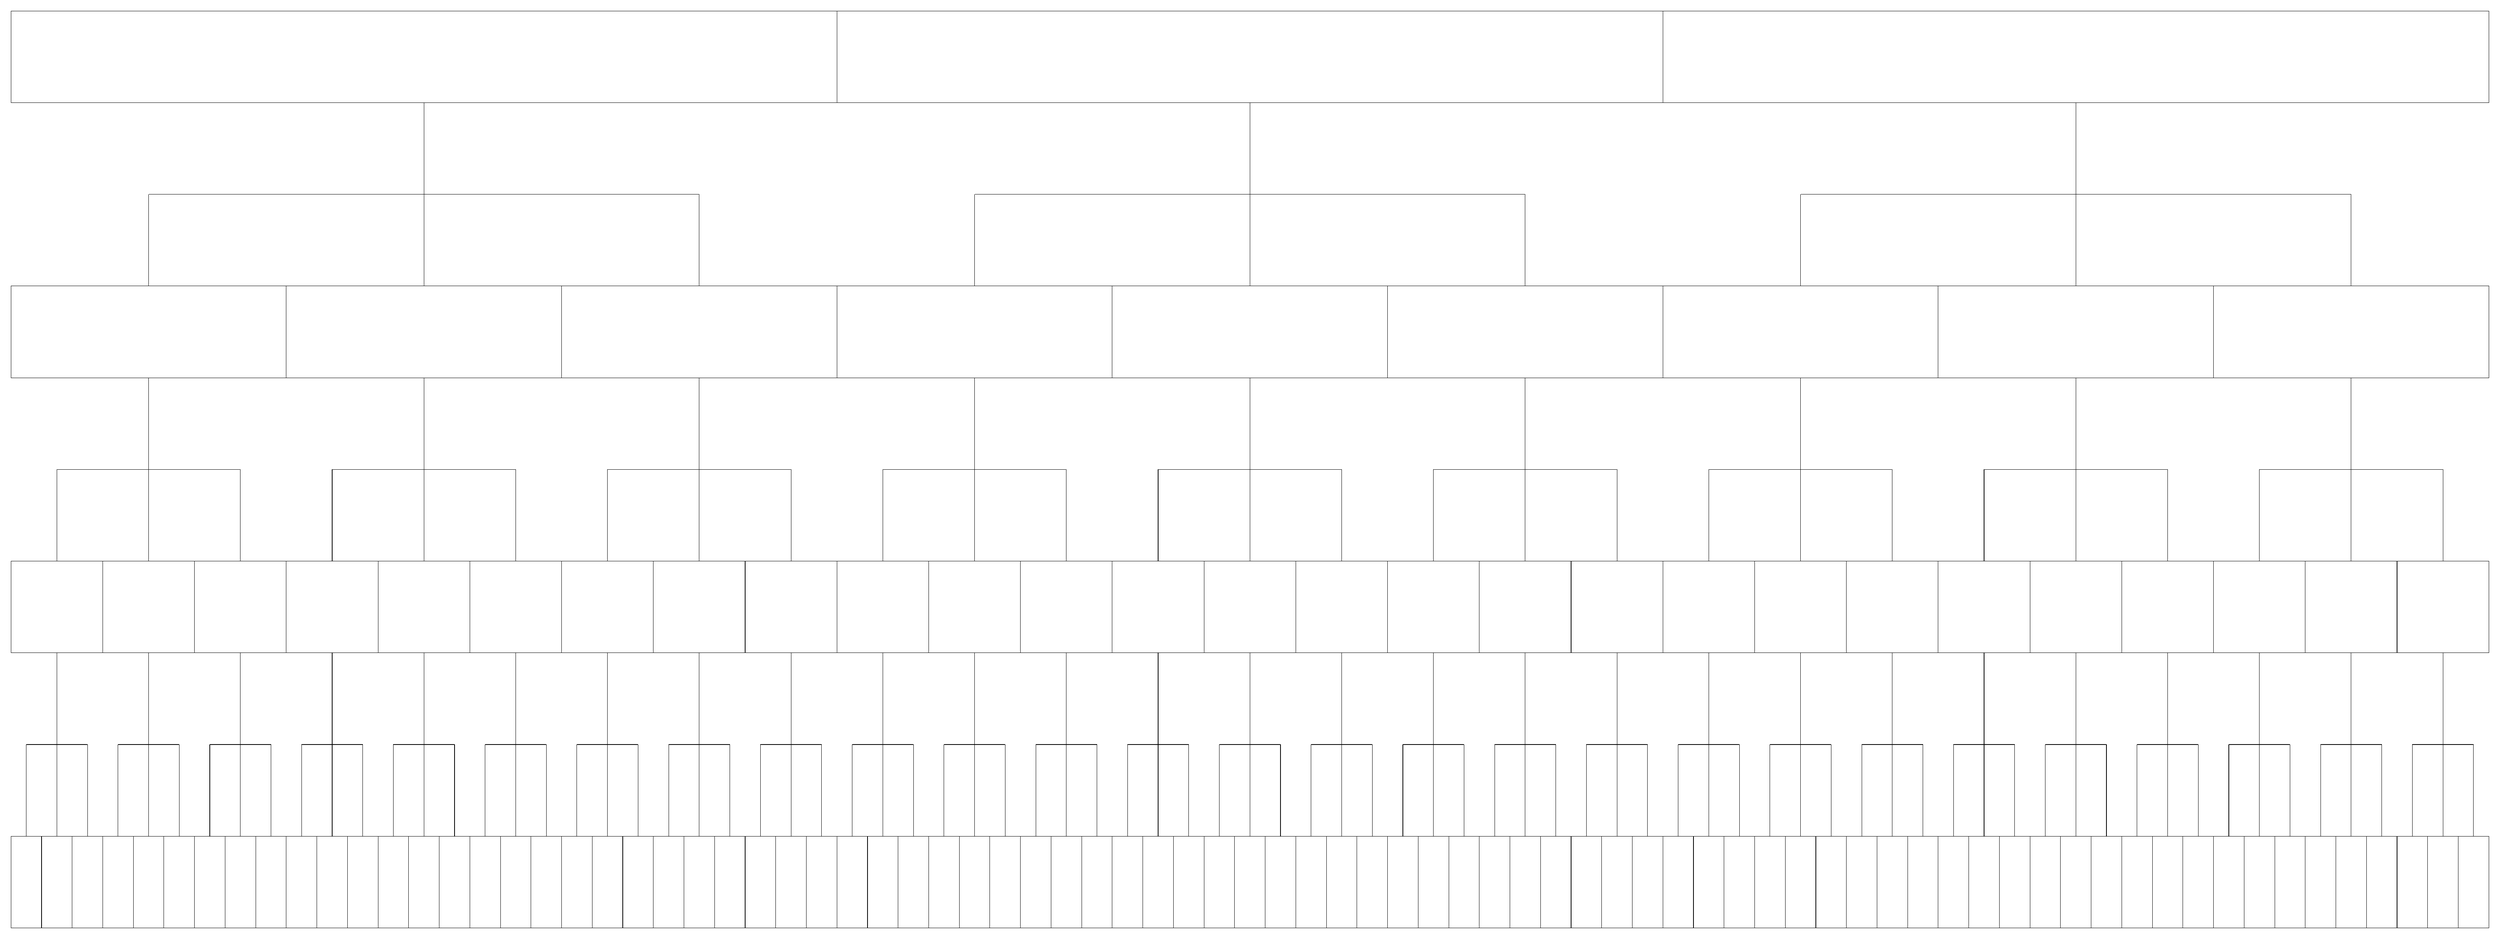
\begin{tikzpicture}
 
% 81 origin
% 27 lvl lmax
% 9 9 9 lvl i
% 3 3 3 lvl 1
% 111  lvl 0
\foreach \r in {3}{%ratio vertical
\foreach \i in {0,1,2} {
    \draw (27 * \i, \r * 0) -- (27 * \i, \r * -1) -- (27 * \i+27, \r * -1) -- (27 * \i+27, \r * 0) -- (27 * \i, \r * 0); 
    \draw (13.5 + 27 * \i, \r * -1) -- (13.5 + 27 * \i, \r * -2);
    \draw (4.5 + 27 * \i, \r * -2) -- (22.5 + 27 * \i, \r * -2);

        
      \foreach \j in {3*\i,3*\i+9,3*\i+18}{
	\draw (9 * \j + 4.5, \r * -2) -- (9 * \j + 4.5, \r * -3);
	\draw (9 * \j, \r * -4) -- (9 * \j, \r * -3) -- (9 * \j+9, \r * -3) -- (9 * \j+9, \r * -4) -- (9 * \j, \r * -4);
	\draw (4.5 + 9 * \j, \r * -4) -- (4.5 + 9 * \j, \r * -5);
        \draw (1.5 + 9 * \j, \r * -5) -- (7.5 + 9 * \j, \r * -5);
        
	\foreach \k in {3*\j,3*\j+3,3*\j+6}{
	  \draw (3 * \k + 1.5, \r * -5) -- (3 * \k + 1.5, \r * -6);
	  \draw (3 * \k, \r * -7) -- (3 * \k, \r * -6) -- (3 * \k+3, \r * -6) -- (3 * \k+3, \r * -7) -- (3 * \k, \r * -7);
	  \draw (1.5 + 3 * \k, \r * -7) -- ( 1.5 + 3 * \k, \r * -8);
	  \draw (0.5 + 3 * \k, \r * -8) -- (2.5 + 3 * \k, \r * -8);
	  
	  \foreach \l in {3*\k,3*\k+1,3*\k+2}{
	    \draw (\l + 0.5, \r * -8) -- (\l + 0.5, \r * -9);
	    \draw (\l, \r * -10) -- (\l, \r * -9) -- (\l+1, \r * -9) -- (\l+1, \r * -10) -- (\l, \r * -10); %faudrait faire des cerlces
% 	    \node[draw=none] at (\l + 0.5, \r * -9.5) {id {\l} };

	  }
	  
	  
	}
    }
}
}
\end{tikzpicture}
